\section{Đặc tả yêu cầu}
Hệ thống điều khiển ánh sáng thông minh (tiếng Anh: Smart Lighting Control System) là một hệ thống tự động điều chỉnh đèn dựa trên điều kiện ánh sáng xung quanh và hỗ trợ người dùng điều khiển thủ công khi cần thiết nhằm tiết kiệm năng lượng điện cũng như có thể vận hành hiệu quả, chính xác mà không cần sự can thiệp của con người.    

\textbf{Yêu cầu: }
\begin{itemize}
    \item Hệ thống gồm 01 đèn LED, 01 cảm biến ánh sáng dùng để điều khiển tự động đèn LED theo điều kiện ánh sáng xung quanh (Auto Mode) và 01 nút bấm dùng để điều khiển thủ công (Manual Mode).
    \item Hệ thống vận hành theo 2 chế độ (mode): Auto Mode và Manual Mode.
    \item Khi bắt đầu chạy thì hệ thống sẽ chạy theo Auto Mode: Đèn LED sẽ tự động tắt (Off) khi trời sáng và sẽ tự động sáng nhấp nháy (Blinking) khi trời tối.
    \item Khi nhấn vào nút bấm thì hệ thống sẽ chuyển từ đổi từ Auto Mode sang Manual Mode: Đèn sẽ tạm thời không vận hành tự động (Auto Mode) theo điều kiện ánh sáng môi trường. Theo đó, nếu người dùng nhấn nút bấm thì đèn sẽ tắt nếu đèn đang sáng và ngược lại, nếu người dùng nhấn nút bấm thì đèn sẽ bật nếu hiện tại đèn đang tắt. Nếu người dùng nhấn nút khi đèn đang blinking thì đèn sẽ tắt. 
    \item Nếu hệ thống đang trong Manual Mode, khi có sự chuyển đổi ánh sáng ngày đêm thì hệ thống sẽ mặc định chuyển về Auto Mode và đèn LED sẽ vận hành tự động theo điều kiện ánh sáng môi trường.
    \item Ngoài ra, khi hệ thống đang trong Manual Mode mà sau N phút người dùng không nhấn nút bấm điều khiển bật tắt đèn thủ công thì hệ thống sẽ tự động chuyển sang Auto Mode. Người dùng có thể thiết lập giá trị N này qua website (Nếu người dùng cài đặt N = 0 thì hệ thống sẽ chỉ chuyển từ Manual Mode sang Auto Mode khi có sự chuyển đổi ánh sáng ngày đêm).
    \item Hệ thống sẽ hỗ trợ website để người dùng theo dõi trạng thái đèn hiện tại (Bật, Tắt, Blinking), mode (Auto Mode hay Manual Mode), điều kiện ánh sáng hiện tại (Light hay Night), điều kiện thời gian N để chuyển mode cho hệ thống. Ngoài ra, người dùng có thể bật, tắt đèn thông qua Website này, cũng như điều chỉnh thông số N (Đơn vị: millisecond).
\end{itemize}

\textbf{Ràng buộc:} 
\begin{itemize}
    \item Hệ thống mô phỏng chỉ được thử nghiệm trên nguồn điện thấp (5-10V), không sử dụng điện dân dụng (220V) để thử nghiệm và vận hành hệ thống này.
    \item Hệ thống không được sử dụng các loại cảm biến thu thập dữ liệu riêng tư của con người dưới mọi hình thức.
    \item Hệ thống luôn phải được cung cấp điện liên tục khi vận hành.
    \item Thiết bị và linh kiện nên phổ biến ở thị trường Việt Nam, có thể dễ dàng tìm kiếm trên địa bàn Thành phố Hồ Chí Minh. Đồng thời ưu tiên sử dụng các thiết bị và linh kiện mà Tinkercad có hỗ trợ mô phỏng.
    \item Chi phí không vượt quá 200.000 VNĐ (bằng chữ: Hai trăm nghìn Việt Nam Đồng chẵn)
\end{itemize}

\section{Thiết kế hệ thống}
\subsection{Thiết kế tổng quát}
\begin{figure}[H]
    \centering
    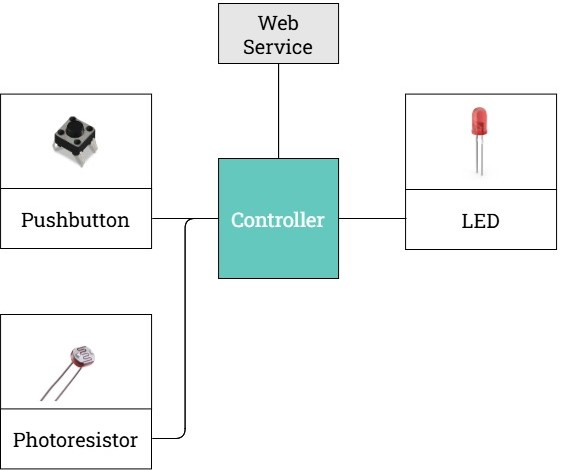
\includegraphics[scale=0.7]{img/SystemDesign.jpg}
    \caption{System Design}
    \label{fig:my_label}
\end{figure}

\subsection{Thiết kế chi tiết}
\begin{table}[h!]
\centering
\small
\begin{tabular}{|p{0.6cm}|p{2.5cm}|p{3.5cm}|p{9cm}|}
\hline
\textbf{TT} & \textbf{Thành phần} & \textbf{Tên thiết bị/Công nghệ đề xuất} & \textbf{Cách thiết lập} \\ \hline
\textbf{1} & Controller & Arduino Uno R3 ATmega328 & 
- Nguồn và GND: Nối chân 5V và GND của Arduino với nguồn điện và GND cho các thiết bị.

- Chân Digital: Nối các thiết bị như LED và Pushbutton vào chân Digital (Pin 2-13) của Arduino để truyền/nhận tín hiệu điều khiển.

- Chân Analog In: Nối cảm biến ánh sáng vào chân Analog In (Pin A0-A5) để đọc tín hiệu ánh sáng.\\ \hline
\textbf{2} & Web Service & Local Host, triển khai bằng Flask, HTML, CSS & 
- Triển khai trên Local Host: Cài đặt Flask trên laptop để tạo server cục bộ.

- Gửi/Nhận Dữ liệu: Thiết lập kết nối giữa Arduino và Web Service thông qua cổng USB của Arduino để trao đổi dữ liệu điều khiển và giám sát trạng thái đèn LED từ Web Service đến Arduino và ngược lại. \\ \hline
\textbf{3} & Pushbutton & 6x6x5 mm Miniature Micro Momentary Tactile Tact Touch Push Button & 
- Kết nối với Arduino: Nối một chân của Pushbutton với chân Digital của Arduino và chân còn lại với GND.

- Điện trở: Thêm điện trở giữa chân Digital và GND để ổn định tín hiệu, tránh nhiễu. Arduino sẽ đọc tín hiệu từ Pushbutton để điều khiển đèn LED.\\ \hline
\textbf{4} & Photoresistor & Lm393 Optical Photosensitive Ldr Light Sensor Module & 
- Kết nối với Arduino: Nối chân tín hiệu của module cảm biến ánh sáng (LDR) với chân Analog In của Arduino. Nối chân VCC và GND của module với chân 5V và GND của Arduino.

- Đọc cường độ ánh sáng: Arduino sẽ đọc giá trị từ LDR để xác định trạng thái sáng tối của môi trường xung quanh. \\ \hline
\textbf{5} & LED & 5mm Color Led & 
- Kết nối với Arduino: Nối chân dương của LED với chân Digital của Arduino qua một điện trở để bảo vệ LED. Nối chân âm của LED với GND.

- Điều khiển Bật/Tắt: Arduino sẽ điều khiển LED dựa trên tín hiệu từ cảm biến ánh sáng hoặc Pushbutton hoặc nhấn nút bật tắt từ Website. \\ \hline
\end{tabular}

\caption{Danh sách các thành phần của hệ thống}
\label{tab:components}

\end{table}

\subsection{Sơ đồ mạch điện đề xuất}
\begin{figure}[H]
    \centering
    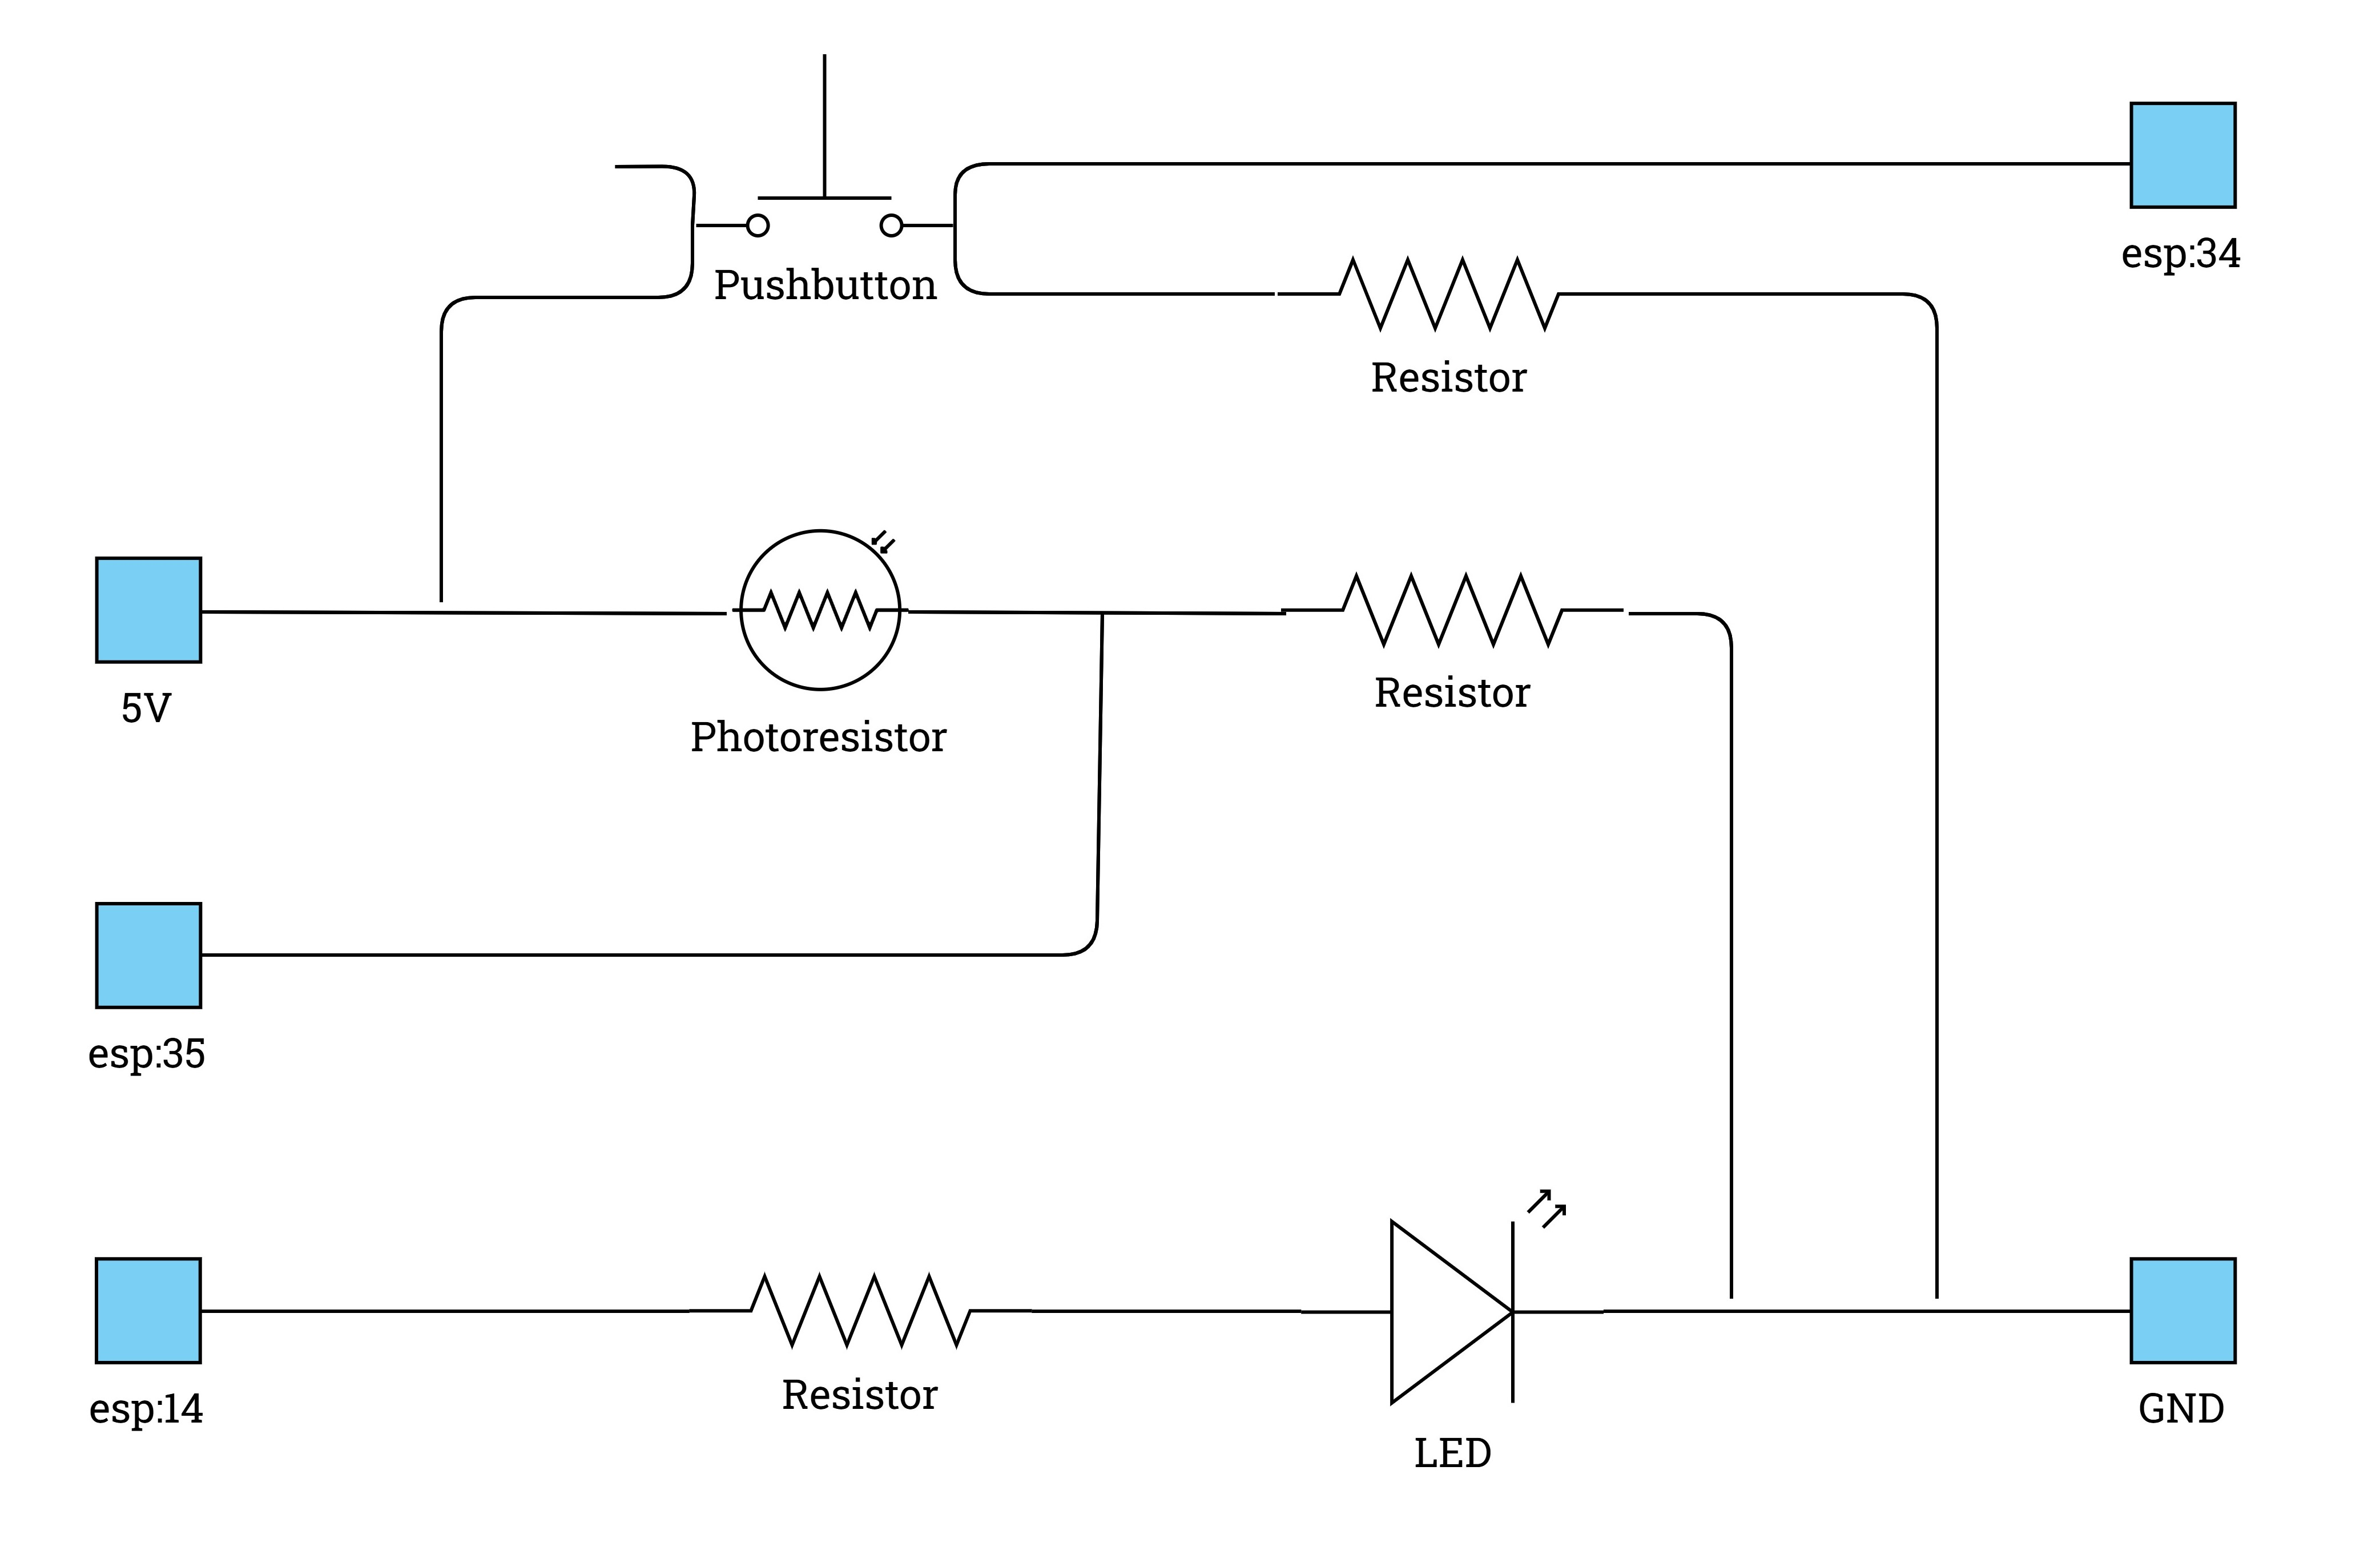
\includegraphics[scale=0.35]{img/Circuit.jpg}
    \caption{Sơ đồ mạch điện dự kiến triển khai hệ thống}
    \label{fig:my_label}
\end{figure}

\subsection{Sơ đồ máy trạng thái hữu hạn (FSM - Finite-state Machine)}
\begin{figure}[H]
    \centering
    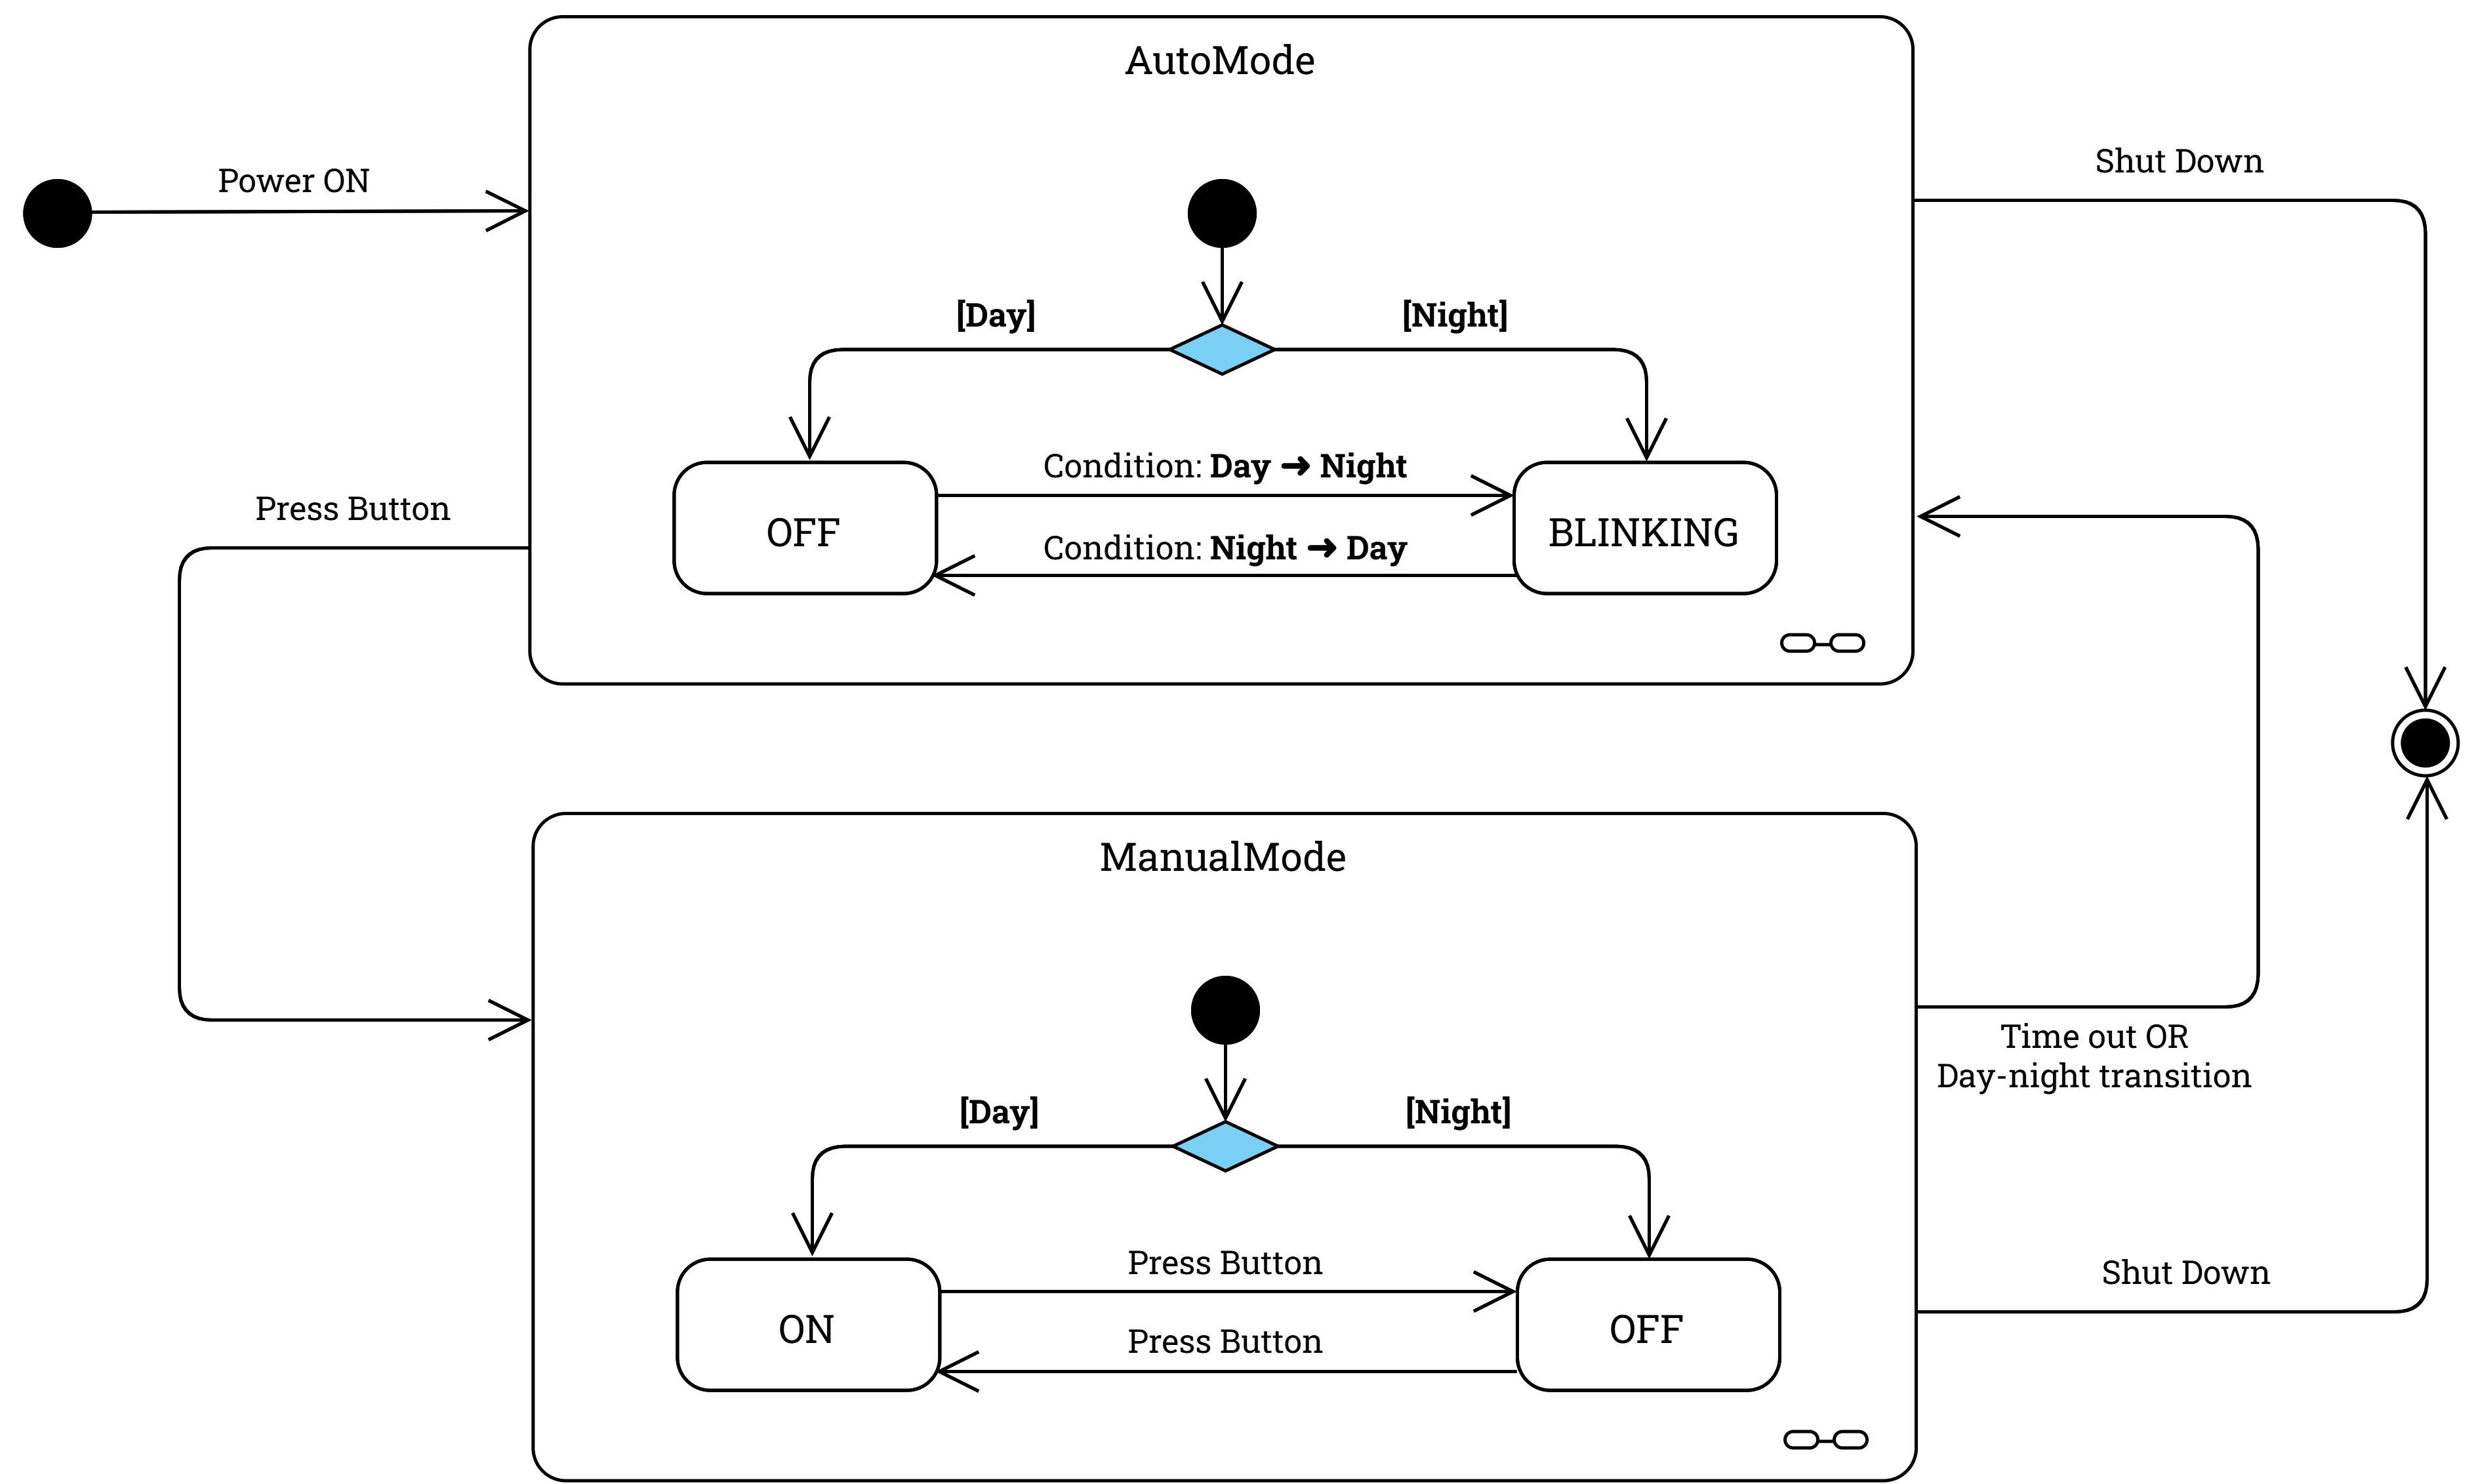
\includegraphics[scale=0.16]{img/FSM-2.jpg}
    \caption{Sơ đồ máy trạng thái hữu hạn của đèn LED trong hệ thống}
    \label{fig:my_label}
\end{figure}

\textbf{Bảng chuyển đổi trạng thái của đèn LED trong hệ thống}

\begin{table}[H]
\centering
\small
\begin{tabular}{|p{2.3cm}|p{3cm}|p{4cm}|p{2cm}|p{4cm}|}
\hline

\textbf{Current State} & \textbf{Input} & \textbf{Condition} & \textbf{Next State} & \textbf{Output} \\ \hline
{Initial State}                                & {Power ON}                            & {Current Condition == Day}                & {AutoMode - OFF}                           & Start AutoMode                            \\ \hline
{Initial State}                                & {Power ON}                            & {Current Condition == Night}              & {AutoMode - BLINKING}                      & Start blinking LED with AutoMode          \\ \hline
{AutoMode - OFF}                               & {Day → Night Transition}              & {-}                                       & {AutoMode - BLINKING}                      & Start blinking LED                        \\ \hline
{AutoMode - BLINKING}                          & {Night → Day Transition}              & {-}                                       & {AutoMode -  OFF}                          & Turn off LED                              \\ \hline
{AutoMode - OFF}                               & {Press Button}                        & {-}                                       & {ManualMode - ON}                          & Switch to ManualMode and turn on LED      \\ \hline
AutoMode - BLINKING                                                 & Press Button                                               & -                                                              & ManualMode - OFF                                                & Switch to ManualMode and turn off LED     \\ \hline
ManualMode - ON                                                     & Press Button                                               & \textit{-}                                                     & ManualMode - OFF                                                & Turn off LED                              \\ \hline
ManualMode - OFF                                                    & Press Button                                               & -                                                              & ManualMode - ON                                                 & Turn on LED                               \\ \hline
ManualMode - ON                                                     & Day-Night Transition                                       & Current Condition == Day                                       & AutoMode - OFF                                                  & Switch to AutoMode and turn off LED       \\ \hline
ManualMode - ON                                                     & Day-Night Transition                                       & Current Condition == Night                                     & AutoMode - BLINKING                                             & Switch to AutoMode and start blinking LED \\ \hline
ManualMode - ON                                                     & Timeout                                                    & Current Condition == Day                                       & AutoMode - OFF                                                  & Switch to AutoMode and turn off LED       \\ \hline
ManualMode - ON                                                     & Timeout                                                    & Current Condition == Night                                     & AutoMode - BLINKING                                             & Switch to AutoMode and start blinking LED \\ \hline
ManualMode - OFF                                                    & Day-Night Transition                                       & Current Condition == Day                                       & AutoMode - OFF                                                  & Switch to AutoMode and turn off LED       \\ \hline
ManualMode - OFF                                                    & Day-Night Transition                                       & Current Condition == Night                                     & AutoMode - BLINKING                                             & Switch to AutoMode and start blinking LED \\ \hline
ManualMode - OFF                                                    & Timeout                                                    & Current Condition == Day                                       & AutoMode - OFF                                                  & Switch to AutoMode and turn off LED       \\ \hline
ManualMode - OFF                                                    & Timeout                                                    & Current Condition == Night                                     & AutoMode - BLINKING                                             & Switch to AutoMode and start blinking LED \\ \hline
AutoMode - OFF                                                      & Shut Down                                                  & -                                                              & -                                                               & Shut Down System                          \\ \hline
AutoMode - BLINKING                                                 & Shut Down                                                  & -                                                              & -                                                               & Shut Down System and turn off LED         \\ \hline
ManualMode - ON                                                     & Shut Down                                                  & -                                                              & -                                                               & Shut Down System and turn off LED         \\ \hline
ManualMode - OFF                                                    & Shut Down                                                  & -                                                              & -                                                               & Shut Down System                          \\ \hline
\end{tabular}
\caption{Bảng chuyển đổi trạng thái của đèn LED trong hệ thống}
\label{tab:my_label}
\end{table}

\subsection{Sơ đồ truyền nhận dữ liệu}
\begin{figure}[H]
    \centering
    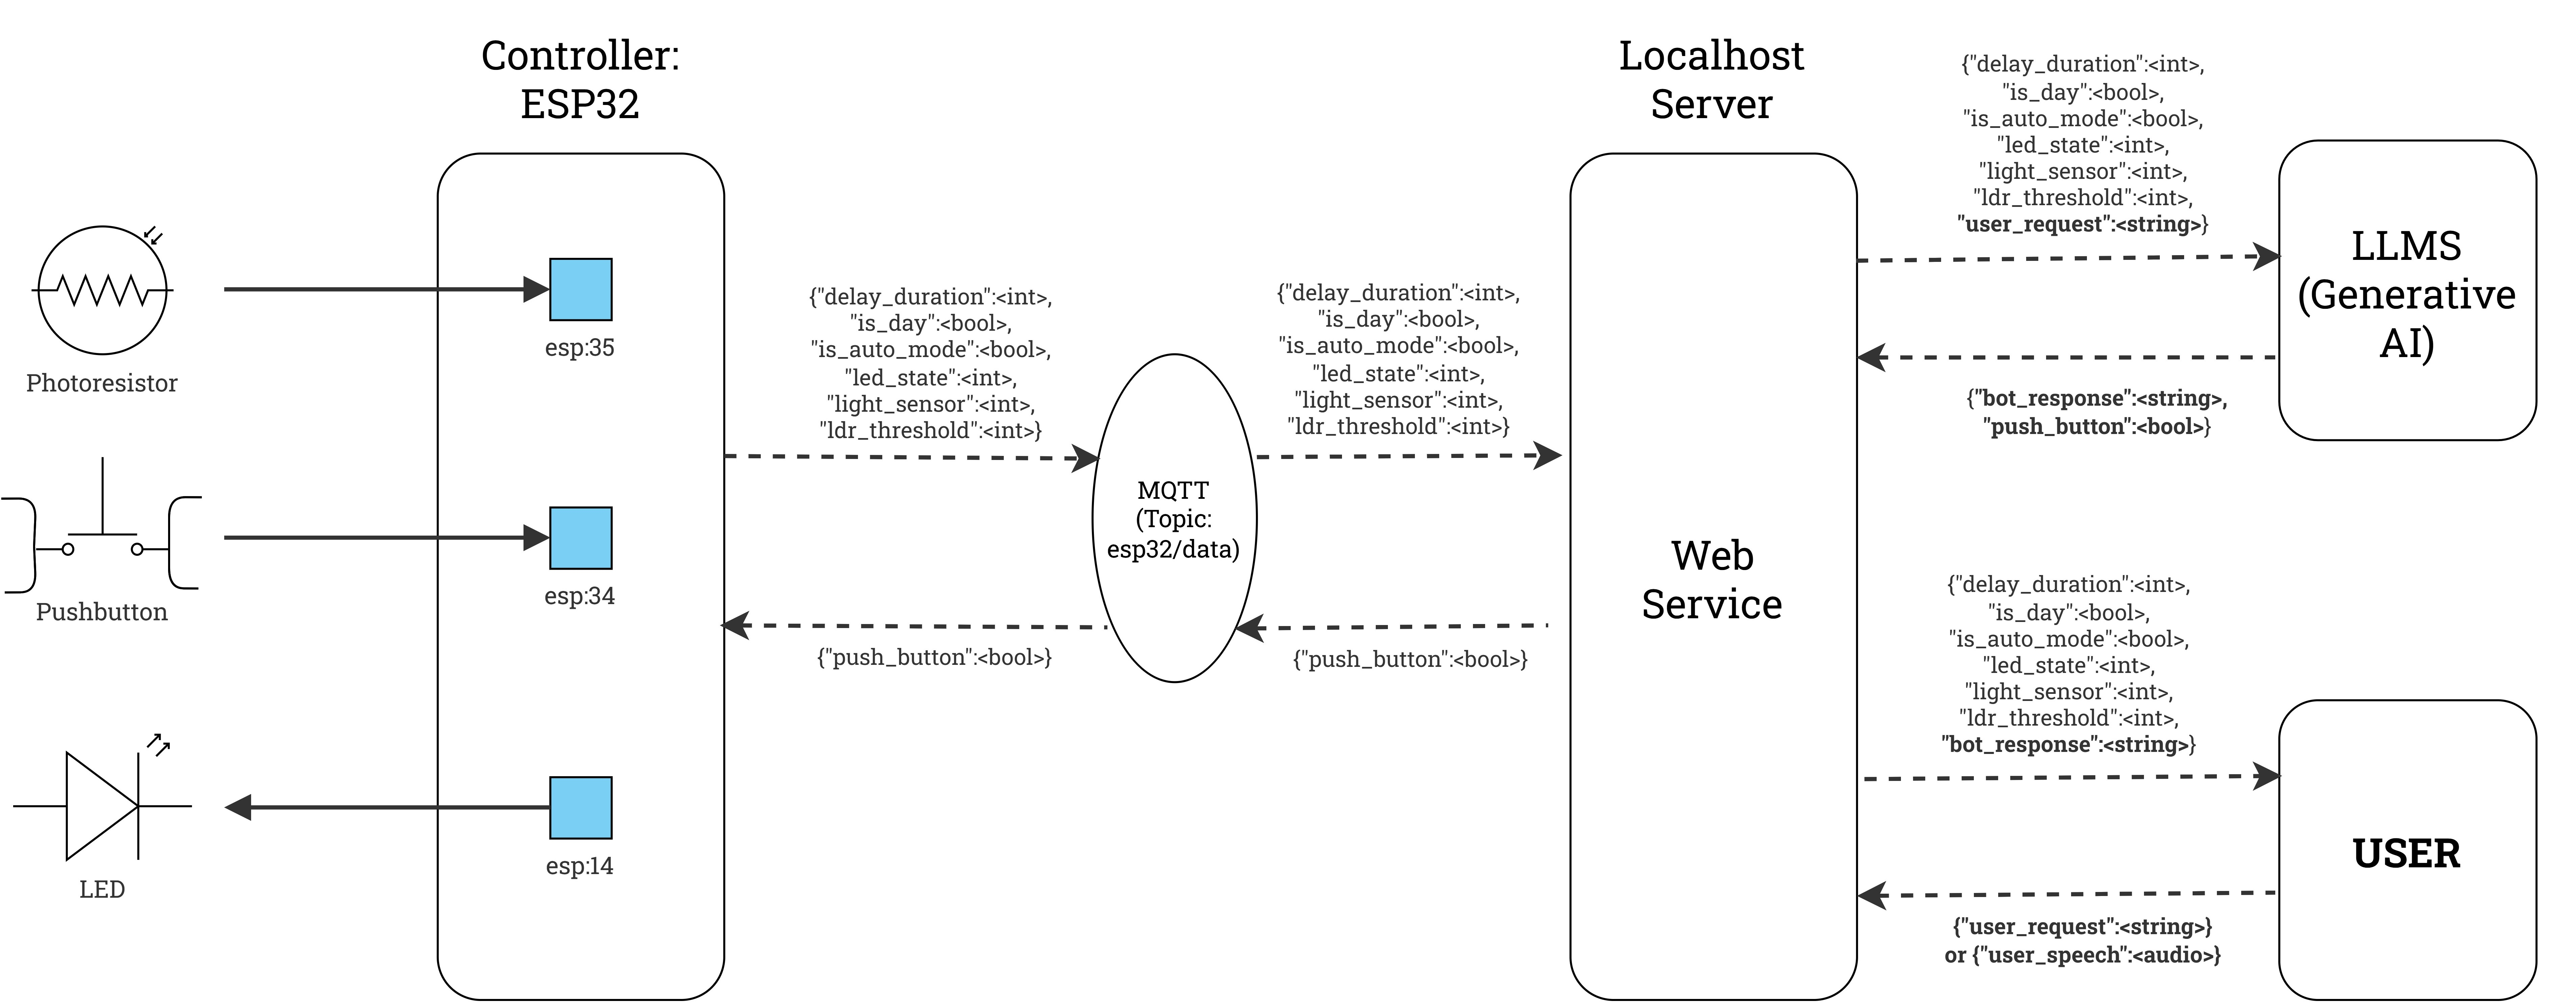
\includegraphics[scale=0.19]{img/Data.jpg}
    \caption{Sơ đồ truyền nhận dữ liệu giữa các thiết bị, Controller và Web Server}
    \label{fig:my_label}
\end{figure}

\subsubsection{Truyền dữ liệu, tín hiệu giữa Controller và các thiết bị}
%\textbf{Các thiết bị truyền dữ liệu, tín hiệu đến Controller:} 
\begin{table}[H]
\centering
\small
\begin{tabular}{|p{2.5cm}|p{2.5cm}|p{2.5cm}|p{2.5cm}|p{4.5cm}|}
\hline
{\textbf{Thiết bị}}            & {\textbf{Pin giao tiếp}} & {\textbf{Điện thế}} & {\textbf{Giá trị}} & {\textbf{Ý nghĩa}}                                 \\ \hline
{Photoresistor}                & {A0}                     & {0V đến 5V}         & {0 đến 1023}       & {Cường độ ánh sáng của môi trường xung quanh hệ thống} \\ \hline
{}                             & {}                       & {0V}                & {LOW}              & {Released}                                         \\ \cline{3-5} 
\multirow{-2}{*}{{Pushbutton}} & \multirow{-2}{*}{{D2}}   & {5V}                & {HIGH}             & {Pressed}                                          \\ \hline

\end{tabular}
\caption{Các thiết bị truyền dữ liệu, tín hiệu đến Controller}
\label{tab:my_label}
\end{table}

%\textbf{Các thiết bị nhận tín hiệu từ Controller: }
\begin{table}[H]
\centering
\small
\begin{tabular}{|p{2.5cm}|p{2.5cm}|p{2.5cm}|p{2.5cm}|p{4.5cm}|}
\hline
{\textbf{Thiết bị}}     & {\textbf{Pin giao tiếp}} & {\textbf{Điện thế}} & {\textbf{Giá trị}} & {\textbf{Ý nghĩa}}         \\ \hline
{}                      & {}                       & {5V}                & {HIGH}             & {ON: tức bật sáng đèn LED} \\ \cline{3-5} 
\multirow{-2}{*}{{LED}} & \multirow{-2}{*}{{D7}}   & {0V}                & {LOW}              & {OFF: tức tắt đèn LED}     \\ \hline
\end{tabular}
\caption{Các thiết bị nhận tín hiệu từ Controller}
\label{tab:my_label}
\end{table}

\pagebreak
\subsubsection{Truyền dữ liệu, tín hiệu từ Controller đến Web Service}
\begin{itemize}
    \item Cấu trúc:
    \begin{lstlisting}
“<switch_mode_duration>,<condition>,<mode>,<blink_state>,<led_state>\n"\end{lstlisting}
    \item Mỗi thông tin cách nhau bởi dấu phẩy, kết thúc chuỗi thông tin gửi bằng dấu “\verb|\n|”
\end{itemize}

\begin{table}[H]
\centering
\small
\begin{tabular}{|p{4cm}|p{5cm}|p{2.5cm}|p{3.5cm}|}
\hline
{\textbf{Trường dữ liệu}}        & {\textbf{Ý nghĩa}}                                                                                                                                                                                                                              & {\textbf{Giá trị gửi}} & {\textbf{Giá trị hiển thị trên Website}}                                  \\ \hline
{switch\_mode\_duration}         & {Thời gian chờ từ lần nhấn nút cuối cùng để hệ thống tự động chuyển từ Manual Mode sang Auto Mode, có thể được người dùng cài đặt trên Website. Lưu ý: nếu đặt giá trị là 0, điều kiện timeout này sẽ không được áp dụng. Đơn vị: millisecond.} & {0 đến 4,294,967,295}  & {0 đến 4,294,967,295 (millisecond)}                                       \\ \hline
{}                               & {}                                                                                                                                                                                                                                              & {0}                    & {Night}                                                                   \\ \cline{3-4} 
\multirow{-2}{*}{condition}    & {Điều kiện ánh sáng của môi trường xung quanh hệ thống (sáng hay tối)}                                                                                                                                                        & {1}                    & {Day/Light}                                                               \\ \hline
{}                               & {}                                                                                                                                                                                                                                              & {0}                    & {Manual}                                                                  \\ \cline{3-4} 
\multirow{-2}{*}{{mode}}         & {{Chế độ hiện tại điều khiển hệ thống là Tự động (Auto) hay Thủ công (Manual)}}                                                                                                                                                 & {1}                    & {Auto}                                                                    \\ \hline
{}                               & {Cho biết đèn LED có đang trong trạng thái chớp nháy hay không.}                                                                                                                                                                                                                                              & {0}                    & {\textit{Not Blinking (thực tế: không hiện trên Website trạng thái này)}} \\ \cline{3-4} 
\multirow{-2}{*}[1.45cm]{{blink\_state}} &{}                                                                                                                                  & {1}                    & {Blinking}                                                                \\ \hline
{}                               & {Cho biết đèn LED có đang tắt hay không.}                                                                                                                                                                                                       & {0}                    & {Off}                                                                     \\ \cline{2-4} 
\multirow{-2}{*}[0.65cm]{{led\_state}}   & {Cho biết đèn LED có đang sáng hay không.}                                                                                                                                                                                                      & {1}                    & {On}                                                                      \\ \hline
\end{tabular}
\caption{Bảng mô tả ý nghĩa của các trường dữ liệu gửi từ Controller đến Web Service}
\label{tab:my_label}
\end{table}

\subsubsection{Truyền dữ liệu, tín hiệu từ Web Service đến Controller}
\begin{itemize}
    \item Cấu trúc:
    \begin{lstlisting}
"<switch_mode_duration>,<is_push_button>\n"\end{lstlisting}
    \item Mỗi thông tin cách nhau bởi dấu phẩy, kết thúc chuỗi thông tin gửi bằng dấu “\verb|\n|”
\end{itemize}

\begin{table}[H]
\centering
\small
\begin{tabular}{|p{4cm}|p{5cm}|p{2.5cm}|p{3.5cm}|}
\hline
{\textbf{Trường dữ liệu}}            & {\textbf{Ý nghĩa}}                                                                                                                                                                                                                              & {\textbf{Giá trị nhập trên Website}} & {\textbf{Giá trị gửi}} \\ \hline
{switch\_mode\_duration}             & {Thời gian chờ từ lần nhấn nút cuối cùng để hệ thống tự động chuyển từ Manual Mode sang Auto Mode, có thể được người dùng cài đặt trên Website. Lưu ý: nếu đặt giá trị là 0, điều kiện timeout này sẽ không được áp dụng. Đơn vị: millisecond.} & {0 đến 4,294,967,295 (millisecond)}       & {0 đến 4,294,967,295}  \\ \hline

\multirow{-2}{*}[-0.25cm]{{is\_push\_button}} & {{Button trên Website có đang được nhấn hay không để bật, tắt đèn LED của hệ thống.}}                                                                                                                                           & {Đang không nhấn}                         & {0}                   \\ \cline{3-4}  {}                                   & {}                                                                                                                                                                                                                                              & {Đã nhấn}                                 & {1}                    
\\ \hline
\end{tabular}
\caption{Bảng mô tả ý nghĩa của các trường dữ liệu gửi từ Web Service đến Controller}
\label{tab:my_label}

\end{table}

\section{Đề xuất các giải pháp}
{% \begin{table}[H]
\centering
\small
\begin{longtable}{|p{2.3cm}|p{3.2cm}|p{3.2cm}|p{3.2cm}|p{3.5cm}|}
\hline
\textbf{Component /Module} & \textbf{Giải pháp 1} & \textbf{Giải pháp 2} & \textbf{Giải pháp 3} & \textbf{Quyết định giải pháp} \\ \hline
\endfirsthead

\hline
\textbf{Component /Module} & \textbf{Giải pháp 1} & \textbf{Giải pháp 2} & \textbf{Giải pháp 3} & \textbf{Quyết định giải pháp} \\ \hline
\endhead

\hline
Controller 
& \textbf{Arduino Uno R3 ATmega328}


- Chi phí: $\sim$100.000 VNĐ


- Dễ lập trình và mở rộng


- Phù hợp cho các hệ thống cơ bản & \textbf{Raspberry Pi 3B+}


- Chi phí: \textgreater{}1.890.000 VNĐ


- Có khả năng xử lý cao hơn


- Hỗ trợ hệ điều hành


- Phù hợp cho các ứng dụng phức tạp & \textbf{ESP32}


- Chi phí: $\sim$150.000 VNĐ


- Tích hợp sẵn Wifi và Bluetooth


- Phù hợp cho IoT và hệ thống có kết nối mạng

& \textbf{Arduino Uno R3 ATmega328}


Đáp ứng đủ yêu cầu, chi phí hợp lý, dễ sử dụng. \\ \hline

Web Service 

& \textbf{Local Host (Flask, HTML, CSS)}


- Triển khai cục bộ trên máy tính


- Chi phí: Miễn phí


- Thích hợp cho giai đoạn thử nghiệm & \textbf{Cloud Hosting}


- Dùng nền tảng đám mây (AWS, Azure)


- Chi phí: phí duy trì hàng tháng


- Khả năng mở rộng tốt


- Truy cập từ xa tiện lợi & \textbf{Raspberry Pi làm Server}


- Kết nối trực tiếp với cảm biến


- Chi phí thiết lập cao hơn


- Phù hợp cho các hệ thống nhỏ gọn, tự chủ & \textbf{Local Host (Flask, HTML, CSS)}


Chi phí thấp và đáp ứng được yêu cầu cơ bản của đồ án. \\ \hline

Pushbutton 

& \textbf{6x6x5 mm Tactile Push Button}


- Chi phí thấp


- Đơn giản, dễ lắp đặt & \textbf{Công tắc cảm ứng chạm}


- Chi phí cao hơn (khoảng 20.000 VNĐ)


- Tạo trải nghiệm hiện đại


- Có thể nhúng vào thiết kế đẹp mắt & \textbf{Công tắc nhấn IP67}


- Chống nước và bụi, phù hợp môi trường ngoài trời


- Chi phí cao hơn (khoảng 20.000 VNĐ)


- Độ bền cao 

& \textbf{6x6x5 mm Tactile Push Button}


Đơn giản, chi phí thấp, dễ sử dụng. \\ \hline

Photoresistor 

& \textbf{Lm393 Optical Photosensitive LDR}


- Chi phí thấp (khoảng 20.000 VNĐ)


- Độ nhạy cao với ánh sáng


- Dễ kết nối với Arduino & \textbf{Cảm biến ánh sáng BH1750}


- Chi phí cao hơn ($\sim$40.000 VNĐ)


- Độ chính xác cao hơn


- Kết nối qua giao thức I2C 

& \textbf{Cảm biến TSL2561}


- Chi phí khoảng  140.000 VNĐ


- Đo ánh sáng với độ chính xác cao, dải rộng


- Phù hợp cho các dự án cần đo ánh sáng chính xác 

& \textbf{Lm393 Optical Photosensitive LDR}


Đáp ứng yêu cầu chi phí thấp và dễ sử dụng trong môi trường ánh sáng đơn giản. \\ \hline

LED 

& \textbf{5mm Color LED}


- Đơn giản, dễ lắp đặt


- Chi phí thấp ($\sim$9.000 VNĐ/30 đèn) 

& \textbf{LED RGB}


- Đổi màu, tạo hiệu ứng


- Chi phí cao hơn ($\sim$16.000 VNĐ)


- Phù hợp nếu cần thay đổi màu sắc 

& \textbf{Grove - LED Button}


- Có tích hợp sẵn kèm theo với Pushbutton.


- Tuổi thọ sử dụng cao hơn (100.000 lần bật tắt)


- Chi phí cao hơn ($\sim$66.000 VNĐ) 

& \textbf{5mm Color LED}


Chi phí thấp, đáp ứng yêu cầu chiếu sáng cơ bản. \\ \hline

\caption{Danh sách đề xuất các giải pháp cho hệ thống}
\label{}
\end{longtable}

% \end{table}
}

\pagebreak
\section{Kế hoạch kiểm thử}
\subsection{Kiểm tra từng thành phần}
\begin{table}[h!]
\centering
\small
\begin{tabular}{|p{4cm}|p{10cm}|}
\hline
\textbf{Thành phần} & \textbf{Kiểm tra} \\ \hline
Controller (Arduino Uno R3 ATmega328) & - Kiểm tra Controller khởi tạo đúng và tất cả các chân (pins) được cấu hình theo thiết kế. \\
& - Kiểm tra giao tiếp nối tiếp dữ liệu Serial giữa Arduino và máy tính thông qua USB Port để đảm bảo khả năng truyền dữ liệu chính xác. \\ \hline
Web Service (Local Host với Flask, HTML, CSS) & - Kiểm tra các route của Flask xử lý yêu cầu và trả về kết quả như mong đợi.


- Giả lập dữ liệu gửi từ Arduino và kiểm tra dữ liệu được nhận và hiển thị chính xác. Đồng thời xuất kết quả gửi từ Flask trên terminal để đảm bảo tính chính xác của dữ liệu gửi đến Arduino. \\ \hline
Pushbutton (6x6x5 mm Miniature Micro Momentary Tactile Tact Push Button) & - Xác nhận nút nhấn ghi nhận trạng thái thay đổi (nhấn và thả) và gửi dữ liệu đến Controller. \\ \hline
Photoresistor (Lm393 Optical Photosensitive LDR Light Sensor Module) & - Đo độ nhạy sáng và đảm bảo đọc giá trị analog chính xác trên chân A0. 


- Kiểm tra khả năng của quang trở để phân biệt giữa ngưỡng sáng ngày và đêm. (Đặc biệt tại môi trường dự kiến triển khai hệ thống) \\ \hline
LED (5mm Color LED) & - Kiểm tra đèn LED phản hồi tín hiệu kỹ thuật số từ chân D7 cho các trạng thái BẬT, TẮT và NHẤP NHÁY. \\
& - Kiểm tra độ sáng/độ rõ của đèn LED trong điều kiện bình thường. \\ \hline
\end{tabular}
\caption{Kiểm tra các thành phần hệ thống}
\label{tab:component_checks}
\end{table}

\pagebreak
\subsection{Kiểm tra tích hợp}

\begin{table}[h!]
\centering
\small
\begin{tabular}{|c|p{4cm}|p{8cm}|}
\hline
\textbf{Bước} & \textbf{Tích hợp} & \textbf{Kiểm tra} \\ \hline
1 & Arduino + Dịch vụ Web & - Kiểm tra phản hồi của dịch vụ web khi Arduino gửi dữ liệu giả lập từ nút nhấn, cảm biến ánh sáng và các dữ liệu kèm theo khác. \\ \hline
3 & Arduino + Dịch vụ Web + Quang trở & - Thay đổi điều kiện ánh sáng xung quanh để kích hoạt quang trở và kiểm tra sự thay đổi trạng thái trên dịch vụ web. \\ \hline
4 & Arduino + Dịch vụ Web + Quang trở + LED & - Kiểm tra đèn LED BẬT, TẮT hoặc NHẤP NHÁY dựa trên đầu vào từ cảm biến ánh sáng, được ghi nhận trên dịch vụ web. \\ \hline
4 & Arduino + Dịch vụ Web + Quang trở + LED + Nút nhấn & - Kiểm tra đèn LED BẬT, TẮT hoặc NHẤP NHÁY dựa trên đầu vào từ nút nhấn, được ghi nhận trên dịch vụ web. \\ \hline
5 & Tích hợp toàn bộ hệ thống & - Thực hiện kiểm tra toàn diện cho cả hệ thống khi tất cả các thành phần hoạt động, đảm bảo hành vi FSM khớp với thiết kế (TẮT, BẬT, NHẤP NHÁY). \\
  & & - Xác nhận trạng thái của đèn LED thay đổi chính xác dựa trên cả nút nhấn vật lý và nút nhấn trên Website cũng như dựa trên đầu vào từ cảm biến ánh sáng, và tất cả dữ liệu được ghi lại trên dịch vụ web. \\
  & & - Xác nhận các thông tin khác hiển thị trên Website được nhận từ Arduino khớp với thực tế. \\ \hline
\end{tabular}
\caption{Các bước tích hợp và kiểm tra hệ thống}
\label{tab:integration_check}
\end{table}

\pagebreak
\section{Kết quả triển khai}
\subsection{Giả lập hệ thống trên Tinkercad }
\begin{figure}[H]
    \centering
    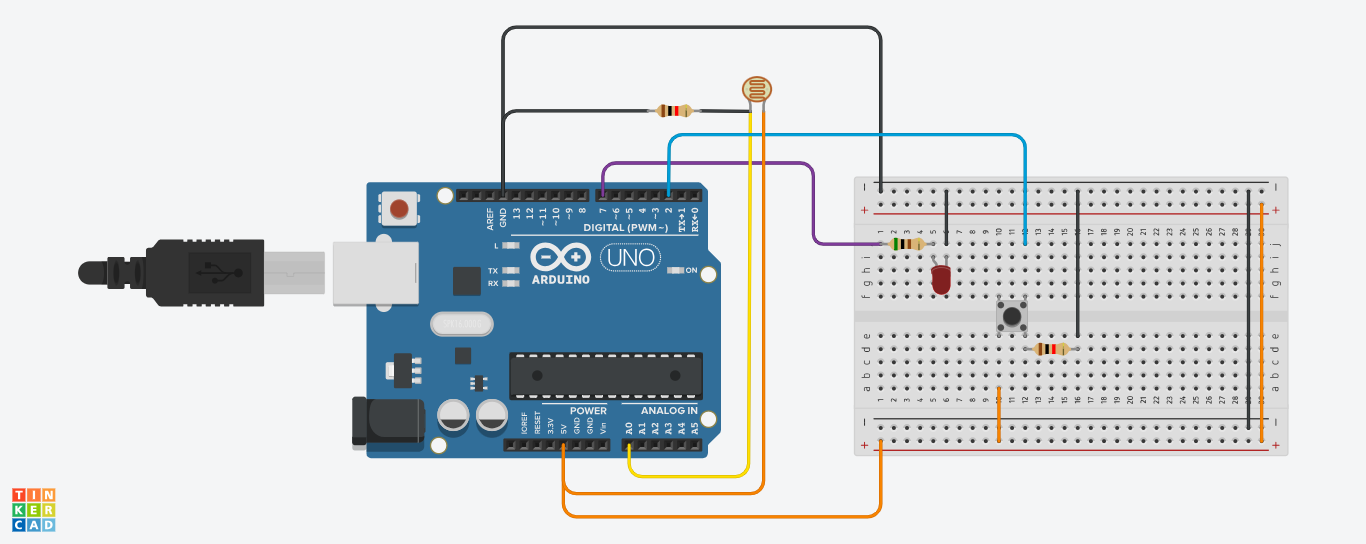
\includegraphics[scale=0.35]{img/Tinkercad.png}
    \caption{Triển khai mạch Arduino trên Tinkercad}
    \label{fig:my_label}
\end{figure}

\subsection{Triển khai hệ thống trên thiết bị thật}
\begin{figure}[H]
    \centering
    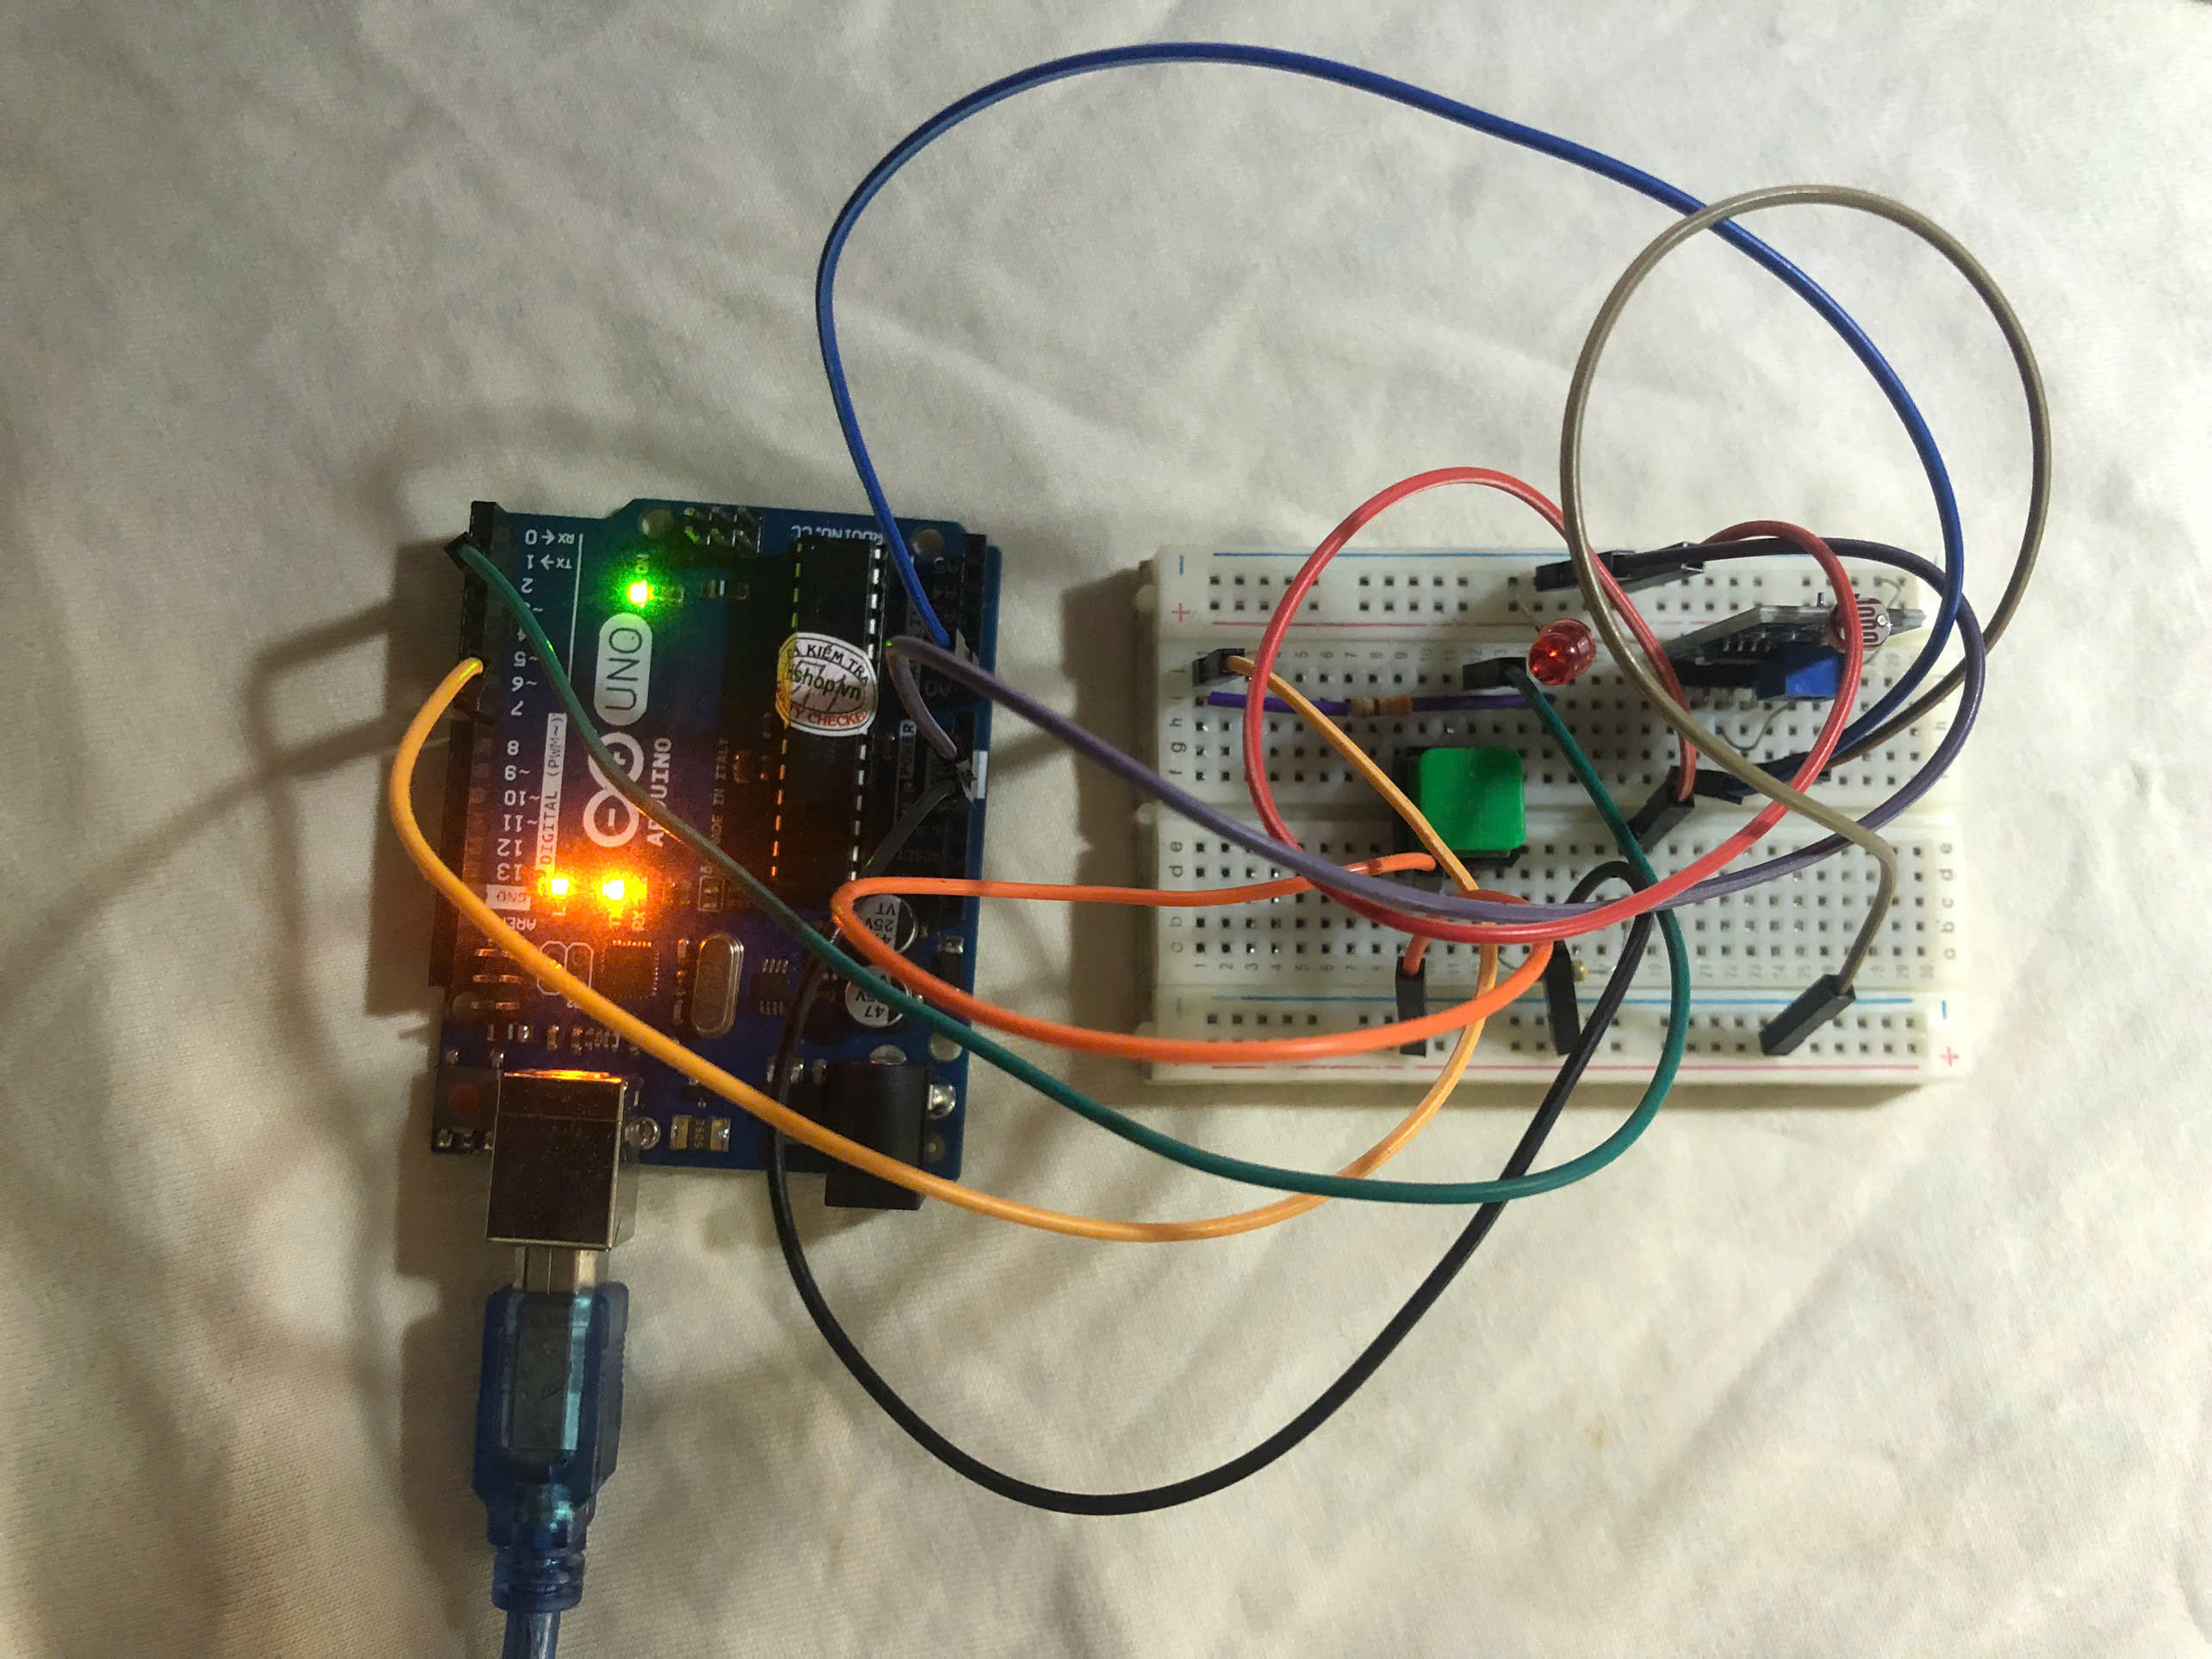
\includegraphics[scale=0.12]{img/realSystem.jpg}
    \caption{Triển khai hệ thống thực tế}
    \label{fig:my_label}
\end{figure}

\begin{figure}[H]
    \centering
    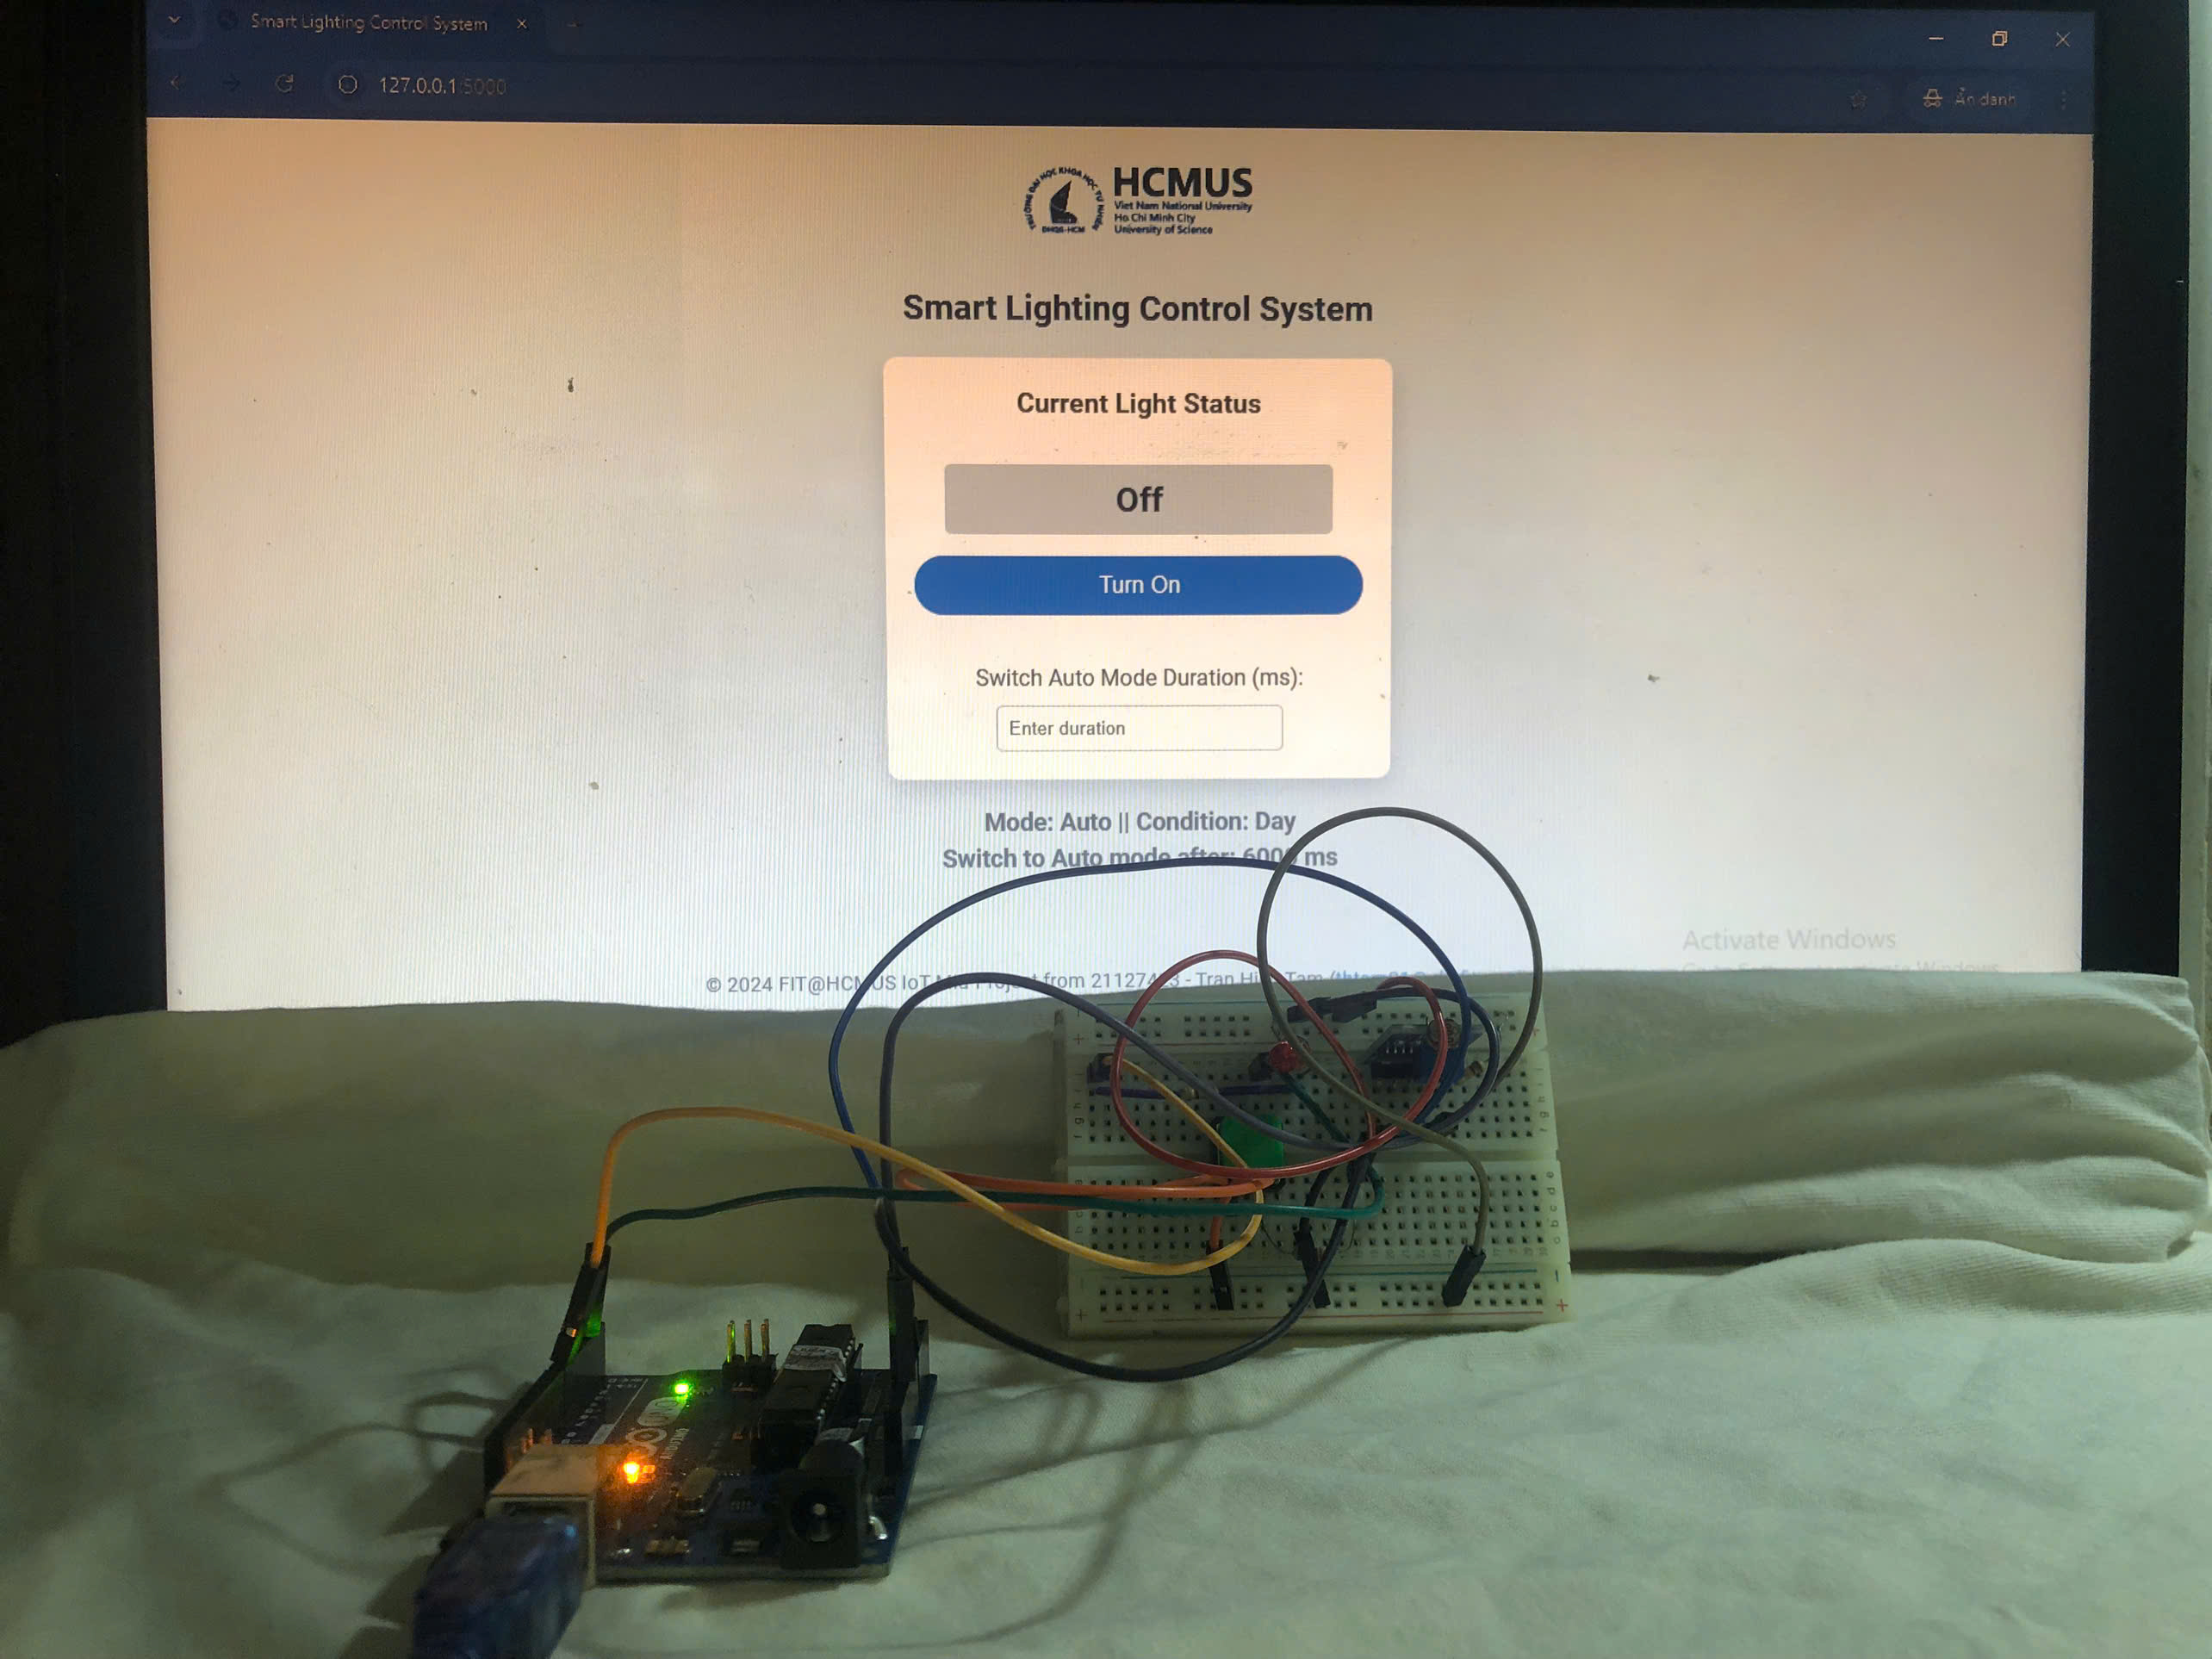
\includegraphics[scale=0.12]{img/SystemWeb.jpg}
    \caption{Triển khai hệ thống thực tế tích hợp Web Service}
    \label{fig:my_label}
\end{figure}

\subsection{Triển khai Website}

{
\centering
\small
\begin{tikzpicture}[
    edge from parent fork down,
    every node/.style={fill=blue!20,rounded corners},
    level 1/.style={sibling distance=5cm},
    level 2/.style={sibling distance=3cm}
  ]
  \node {Source}
    child { node {IoT-SmartLighting}
      child { node {IoT-SmartLighting.ino} }
    }
    child { node {static}
      child { node {images} {child {node {Logo-HCMUS.png} }}}
      child { node {style.css} }
    }
    child { node {templates}
      child { node {index.html} }
    }
    child { node {app.py} };
\end{tikzpicture}
}
\begin{itemize}
    \item \textbf{Bước 1:} Cài đặt Python, Flask và các thư viện liên quan
    \item \textbf{Bước 2:} Lập trình và tổ chức các file sau

    \begin{itemize}
        \item Source\textbackslash IoT-SmartLighting\textbackslash IoT-SmartLighting.ino: Đây là file mã nguồn cho Arduino, được viết bằng ngôn ngữ C/C++ trong môi trường Arduino IDE. File này chứa các đoạn mã để điều khiển các phần cứng trong hệ thống Smart Lighting, như đọc dữ liệu từ cảm biến ánh sáng, điều khiển đèn LED, và xử lý nút bấm.
        \item Source\textbackslash static\textbackslash images\textbackslash Logo-HCMUS.png: Hình ảnh hiển thị trên website. 
        \item Source\textbackslash static\textbackslash style.css: File CSS này chứa các quy tắc và định dạng giao diện cho trang web. Nó quy định cách thức hiển thị các thành phần như màu sắc, phông chữ, bố cục, và phong cách của trang web.
        \item Source\textbackslash templates\textbackslash index.html: Đây là file HTML chính để tạo giao diện người dùng cho ứng dụng web. File này chứa cấu trúc của trang web, nơi người dùng có thể tương tác với hệ thống IoT để điều khiển cũng như theo dõi trạng thái hiện tại của đèn LED. 
        \item Source\textbackslash app.py: Đây là file Python chứa mã nguồn cho web server của ứng dụng, được xây dựng bằng Flask framework. File này xử lý các yêu cầu từ trình duyệt web, giao tiếp với Arduino để nhận dữ liệu cảm biến và gửi lệnh điều khiển đến các thiết bị. Nó là thành phần quan trọng giúp kết nối giữa người dùng và phần cứng của hệ thống IoT.
    \end{itemize}

    \item \textbf{Bước 3:} Sử dụng Arduino IDE để nạp code .ino vào Controller. 
    \item \textbf{Bước 4:} Kết nối Arduino (đã được nạp code trước) với Laptop thông qua USB Port. Lưu ý, không mở ứng dụng khác sử dụng chung port với Flask đang chạy. 
    \item \textbf{Bước 5:} Chạy localhost thông qua cmd từ folder Source
    \begin{lstlisting}
flask --app app run\end{lstlisting}
    \item \textbf{Bước 6:} Xem trên Localhost và Terminal
    \begin{lstlisting}
http://127.0.0.1:5000/\end{lstlisting}

\end{itemize}
\begin{figure}[!h]
    \centering
    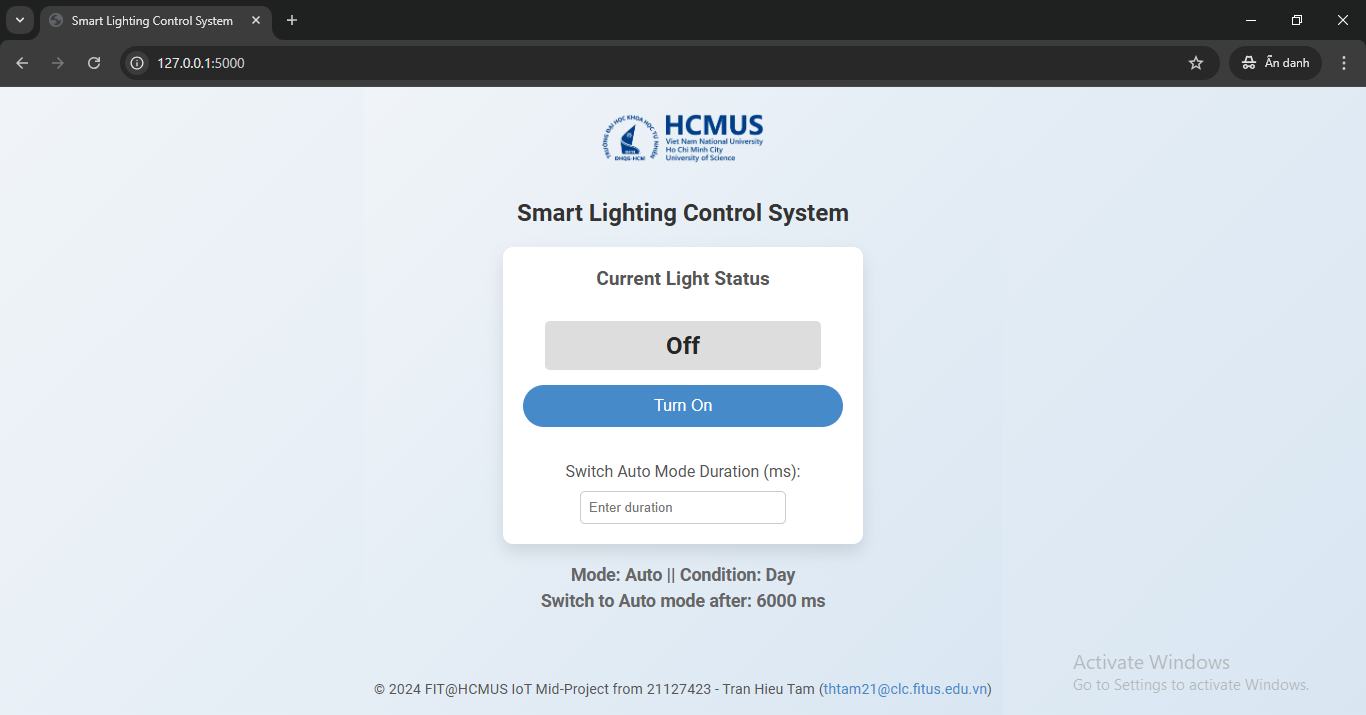
\includegraphics[width=0.75\linewidth]{img/WebUXUI.png}
    \caption{Giao diện Web Service sau khi kết nối với Web Server thành công}
    \label{fig:enter-label}
\end{figure}

\subsection{Giới thiệu chức năng website}
Website gồm có các chức năng sau: 
\begin{itemize}
    \item Theo dõi trạng thái đèn bao gồm Off, On và Blinking.
    \item Theo dõi chế độ vận hành hệ thống hiện tại (Auto Mode hay Manual Mode), trạng thái ánh sáng môi trường xung quanh hệ thống (Day hay Night), timeout từ Manual Mode sang Auto Mode bao nhiêu Millisecond (nếu hiển thị 0 thì hệ thống sẽ bỏ qua điều kiện timeout này khi vận hành)
    \item Khi nhấn vào nút bấm trên Website thì nó vận hành giống như nút bấm vật lý thực tế của hệ thống (thay đổi trạng thái hiện tại của đèn LED trong Manual Mode từ On sang Off, Off sang On, Blinking sang Off).
    \item Khi nhập giá trị vào Switch to Auto Mode Duration và Enter thì giá trị sẽ được gửi cho hệ thống theo đơn vị Millisecond, không tác động đến trạng thái nút bấm trên Website. Nếu nhập vào giá trị 0 thì hệ thống mặc nhiên bỏ điều kiện này khi vận hành.
\end{itemize}

\begin{figure}[!h]
    \centering
    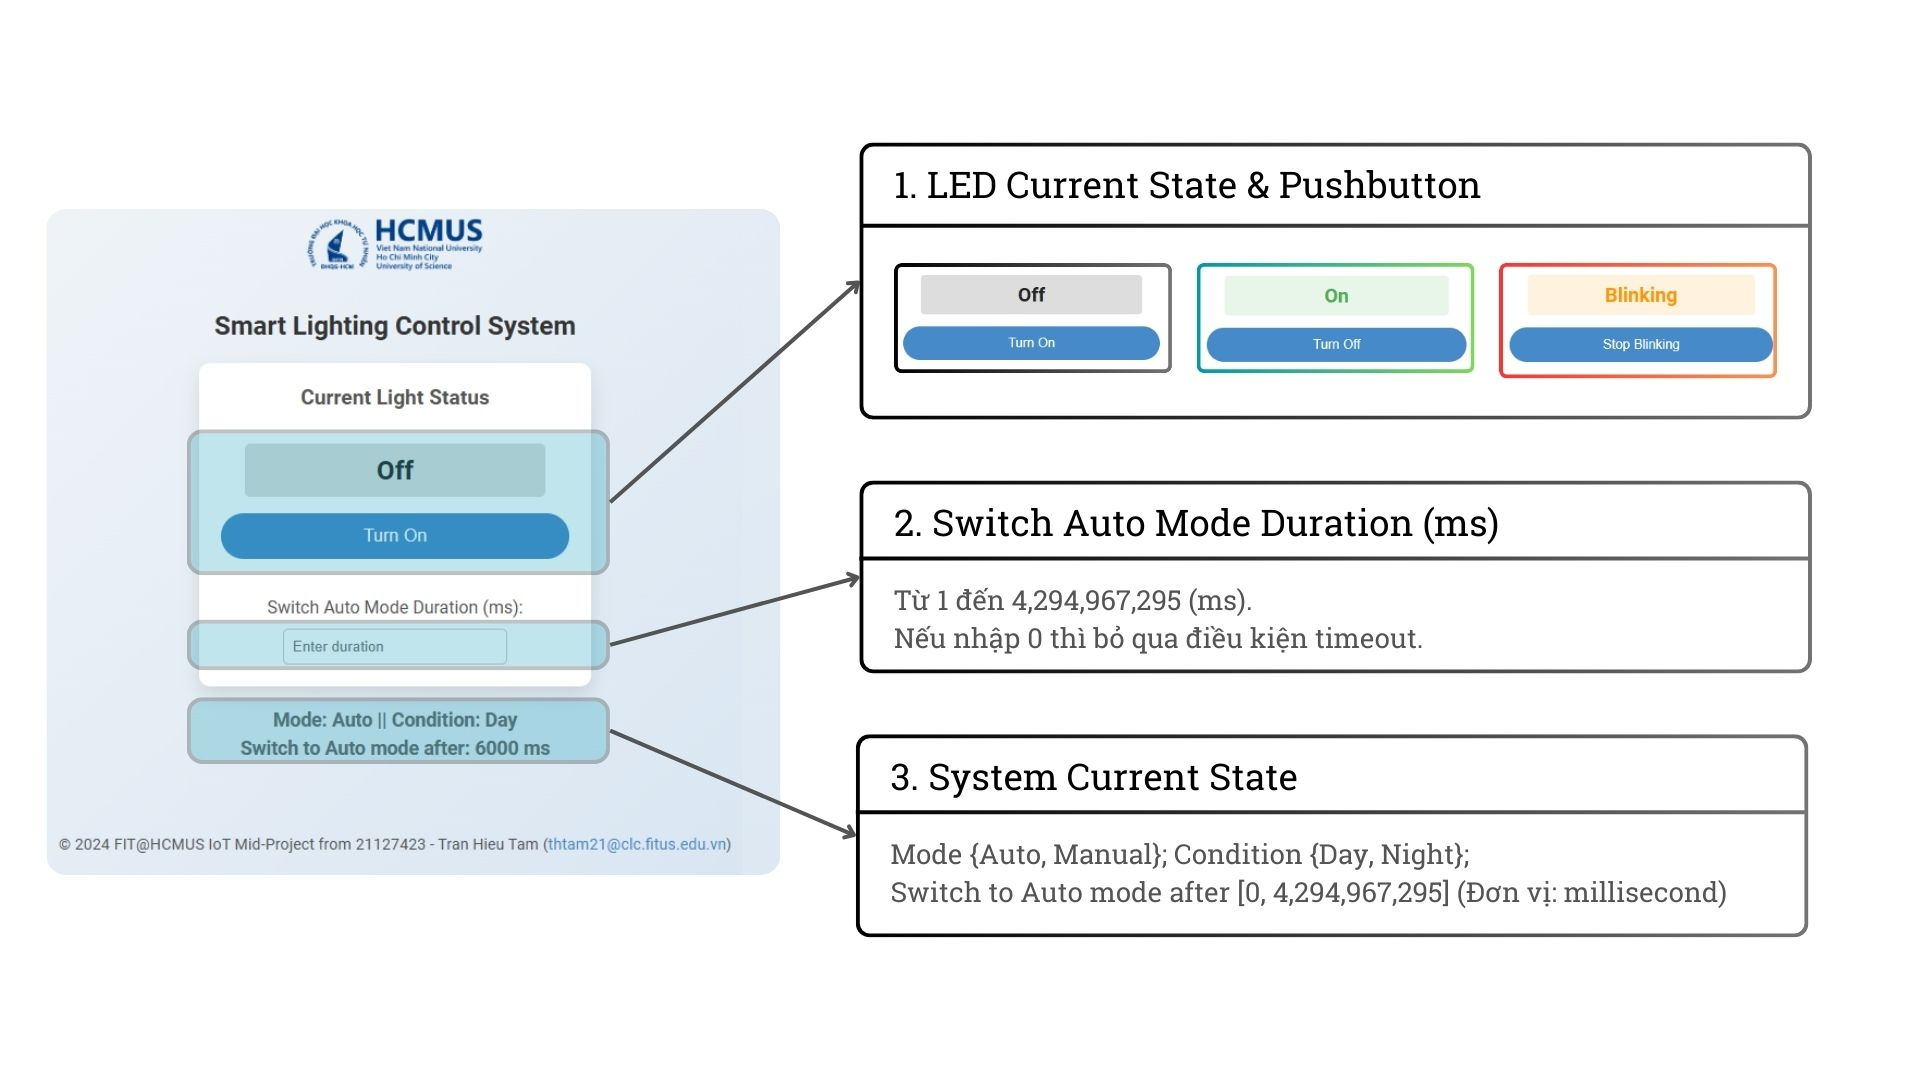
\includegraphics[width=0.8\linewidth]{img/Web.jpg}
    \caption{Các thành phần chính của Website}
    \label{fig:enter-label}
\end{figure}

\subsection{Release}
\begin{lstlisting}[escapeinside={(*@}{@*)}]
21127423,Tran Hieu Tam,(*@\href{https://www.youtube.com/watch?v=MielNnFK-BU}{https://www.youtube.com/watch?v=MielNnFK-BU}@*),(*@\href{https://drive.google.com/drive/folders/1Cm12i8CtkhcVk8lisDeS54gof4zHMSak?usp=sharing}{https://drive.google.com/drive/folders/1Cm12i8CtkhcVk8lisDeS54gof4zHMSak?usp=sharing}@*)
\end{lstlisting}

% Author: Trần Hiếu Tâm

% Contact email: \href{thtam21@clc.fitus.edu.vn}{thtam21@clc.fitus.edu.vn}

% Release date: November 11th, 2024

% Release version: 1.0

% Location: Ho Chi Minh City, Viet Nam

% Copyright: Faculty of Information Technology, VNUHCM - University of Science

% GitHub repository: \href{https://github.com/HieuTam/HCMUS-IoT-SmartLightingControlSystem}{https://github.com/HieuTam/HCMUS-IoT-SmartLightingControlSystem}


\vspace{1cm}
{\small
\subsubsection*{Project Information}

\begin{itemize}
    \item \textbf{Release Version:} 1.0
    \item \textbf{Release Date:} November 11, 2024
    \item \textbf{Author:} Trần Hiếu Tâm
    \item \textbf{Contact Email:} \href{mailto:thtam21@clc.fitus.edu.vn}{thtam21@clc.fitus.edu.vn}
    \item \textbf{Location:} Ho Chi Minh City, Viet Nam
    \item \textbf{GitHub Repository:} \href{https://github.com/HieuTam/HCMUS-IoT-SmartLightingControlSystem}{https://github.com/HieuTam/HCMUS-IoT-SmartLightingControlSystem}\\[1cm]
\end{itemize}

\subsubsection*{Copyright}
\noindent Faculty of Information Technology, VNUHCM-University of Science
}\\[1.5cm]

\begin{figure}[H]
    \centering
    
\includegraphics[width=0.35\linewidth]{img/Logo-HCMUS-Symbol.png}
\end{figure}